\documentclass[12pt]{article}
\usepackage{amsmath}
\usepackage{latexsym}
\usepackage{amsfonts}
\usepackage[normalem]{ulem}
\usepackage{array}
\usepackage{amssymb}
\usepackage{graphicx}
\usepackage[backend=biber,
style=numeric,
sorting=none,
isbn=false,
doi=false,
url=false,
]{biblatex}\addbibresource{bibliography.bib}

\usepackage{subfig}
\usepackage{wrapfig}
\usepackage{wasysym}
\usepackage{enumitem}
\usepackage{adjustbox}
\usepackage{ragged2e}
\usepackage[svgnames,table]{xcolor}
\usepackage{tikz}
\usepackage{longtable}
\usepackage{changepage}
\usepackage{setspace}
\usepackage{hhline}
\usepackage{multicol}
\usepackage{tabto}
\usepackage{float}
\usepackage{multirow}
\usepackage{makecell}
\usepackage{fancyhdr}
\usepackage[toc,page]{appendix}
\usepackage[hidelinks]{hyperref}
\usetikzlibrary{shapes.symbols,shapes.geometric,shadows,arrows.meta}
\tikzset{>={Latex[width=1.5mm,length=2mm]}}
\usepackage{flowchart}\usepackage[paperheight=11.69in,paperwidth=8.28in,left=0.53in,right=0.53in,top=0.56in,bottom=0.19in,headheight=1in]{geometry}
\usepackage[utf8]{inputenc}
\usepackage[T1]{fontenc}
\TabPositions{0.5in,1.0in,1.5in,2.0in,2.5in,3.0in,3.5in,4.0in,4.5in,5.0in,5.5in,6.0in,6.5in,7.0in,}

\urlstyle{same}


 %%%%%%%%%%%%  Set Depths for Sections  %%%%%%%%%%%%%%

% 1) Section
% 1.1) SubSection
% 1.1.1) SubSubSection
% 1.1.1.1) Paragraph
% 1.1.1.1.1) Subparagraph


\setcounter{tocdepth}{5}
\setcounter{secnumdepth}{5}


 %%%%%%%%%%%%  Set Depths for Nested Lists created by \begin{enumerate}  %%%%%%%%%%%%%%


\setlistdepth{9}
\renewlist{enumerate}{enumerate}{9}
		\setlist[enumerate,1]{label=\arabic*)}
		\setlist[enumerate,2]{label=\alph*)}
		\setlist[enumerate,3]{label=(\roman*)}
		\setlist[enumerate,4]{label=(\arabic*)}
		\setlist[enumerate,5]{label=(\Alph*)}
		\setlist[enumerate,6]{label=(\Roman*)}
		\setlist[enumerate,7]{label=\arabic*}
		\setlist[enumerate,8]{label=\alph*}
		\setlist[enumerate,9]{label=\roman*}

\renewlist{itemize}{itemize}{9}
		\setlist[itemize]{label=$\cdot$}
		\setlist[itemize,1]{label=\textbullet}
		\setlist[itemize,2]{label=$\circ$}
		\setlist[itemize,3]{label=$\ast$}
		\setlist[itemize,4]{label=$\dagger$}
		\setlist[itemize,5]{label=$\triangleright$}
		\setlist[itemize,6]{label=$\bigstar$}
		\setlist[itemize,7]{label=$\blacklozenge$}
		\setlist[itemize,8]{label=$\prime$}



 %%%%%%%%%%%%  Header here  %%%%%%%%%%%%%%


\pagestyle{fancy}
\fancyhf{}
\cfoot{ }
\renewcommand{\headrulewidth}{0pt}
\setlength{\topsep}{0pt}\setlength{\parindent}{0pt}
\renewcommand{\arraystretch}{1.3}


%%%%%%%%%%%%%%%%%%%% Document code starts here %%%%%%%%%%%%%%%%%%%%



\begin{document}
\begin{adjustwidth}{1.73in}{1.73in}
\begin{Center}
{\fontsize{17pt}{20.4pt}\selectfont Diseño de Software\par}
\end{Center}\par

\end{adjustwidth}

\begin{adjustwidth}{2.99in}{2.99in}
\begin{Center}
{\fontsize{17pt}{20.4pt}\selectfont Taller No. 1\par}
\end{Center}\par

\end{adjustwidth}

\begin{adjustwidth}{1.2in}{1.2in}
\begin{Center}
{\fontsize{17pt}{20.4pt}\selectfont M´etodos de Ordenamiento\par}
\end{Center}\par

\end{adjustwidth}


\vspace{\baselineskip}
\begin{adjustwidth}{0.0in}{2.47in}
\begin{FlushRight}
Michael Daniel Murillo López
\end{FlushRight}\par

\end{adjustwidth}

\begin{adjustwidth}{2.79in}{2.79in}
\begin{Center}
Ingenier´$\iota$ a de Sistemas
\end{Center}\par

\end{adjustwidth}

\begin{adjustwidth}{2.08in}{2.08in}
\begin{Center}
Corporación Universitaria Minuto de Dios
\end{Center}\par

\end{adjustwidth}

\begin{adjustwidth}{2.08in}{2.08in}
\begin{Center}
30 de A
\end{Center}\par

\end{adjustwidth}


\vspace{\baselineskip}

\vspace{\baselineskip}
\begin{adjustwidth}{0.07in}{0.05in}
\begin{justify}
{\fontsize{11pt}{13.2pt}\selectfont .\par}
\end{justify}\par

\end{adjustwidth}

\begin{adjustwidth}{0.07in}{0.05in}
\begin{justify}
{\fontsize{11pt}{13.2pt}\selectfont Como parte de un ejercicio típico de Desarrollo de algoritmos de software, hice un pequeño análisis comparativo de los algoritmos de ordenamiento más populares, buscando estudiar la complejidad de cada uno de estos y como las diferentes formas de resolver un mismo problema pueden afectar los tiempos de ejecución. Quiero aclarar que este es solo un análisis académico muy simple que quiero documentar, el cual tal vez sirva a futuro para otros estudiantes de ciencias de la computación.\par}
\end{justify}\par

\end{adjustwidth}


\vspace{\baselineskip}
\begin{adjustwidth}{0.07in}{0.05in}
\begin{justify}
{\fontsize{11pt}{13.2pt}\selectfont El usuario debe poder ingresar una serie de números separados por comas, y estos se entenderán como el conjunto de números del arreglo, y usando un menú en la consola debe poder seleccionar cual algoritmo utilizar.\par}
\end{justify}\par

\end{adjustwidth}


\vspace{\baselineskip}

\vspace{\baselineskip}
\begin{adjustwidth}{0.07in}{5.67in}
\begin{justify}
{\fontsize{14pt}{16.8pt}\selectfont 1\   Bubble  Sort:\par}
\end{justify}\par

\end{adjustwidth}


\vspace{\baselineskip}
\begin{adjustwidth}{0.07in}{0.04in}
\begin{justify}
{\fontsize{11pt}{13.2pt}\selectfont Este es uno de los algoritmos mas simples de ordenamiento. Este algoritmo\  se basa en la comparaci´on de el- ementos,\  particularmente entre parejas adyacentes, y si la pareja a comparar no est´a ordenada, simplemente se intercambian; el algoritmo  concluye cuando  al hacer  todo el recorrido,  y hacer  todas  las comparaciones entre  vecinos adyacentes, no se requieren  realizar  mas  intercambios.  Este  algoritmo  no es recomendable para arreglos con gran cantidad de datos,  ya que tanto su caso promedio como su peor caso tienen un orden de crecimiento  de $ \Theta $ (n{\fontsize{8pt}{9.6pt}\selectfont 2{\fontsize{11pt}{13.2pt}\selectfont ).\par}\par}\par}
\end{justify}\par

\end{adjustwidth}


\vspace{\baselineskip}
\begin{adjustwidth}{0.31in}{4.32in}
\begin{justify}
{\fontsize{11pt}{13.2pt}\selectfont Data: A : Unsorted  array  of numbers Result: A$\ast$  : Sorted\  array  of numbers for  i $ \leftarrow $  0 to length(A) $-$  1 do\par}
\end{justify}\par

\end{adjustwidth}

\begin{adjustwidth}{0.54in}{0.0in}
{\fontsize{11pt}{13.2pt}\selectfont swapped  $ \leftarrow $  false\par}\par

\end{adjustwidth}

\begin{adjustwidth}{0.54in}{0.0in}
{\fontsize{11pt}{13.2pt}\selectfont for  j $ \leftarrow $  0 to length(A) $-$  1 do\par}\par

\end{adjustwidth}

\begin{adjustwidth}{0.77in}{0.0in}
{\fontsize{11pt}{13.2pt}\selectfont /$\ast$  compare  to adjacent  elements $\ast$ /\par}\par

\end{adjustwidth}

\begin{adjustwidth}{0.77in}{0.0in}
{\fontsize{11pt}{13.2pt}\selectfont if array[j]  > array[j  + 1] then\par}\par

\end{adjustwidth}

\begin{adjustwidth}{1.01in}{0.0in}
{\fontsize{11pt}{13.2pt}\selectfont /$\ast$  swap them $\ast$ /\par}\par

\end{adjustwidth}

\begin{adjustwidth}{1.01in}{4.68in}
{\fontsize{11pt}{13.2pt}\selectfont auxSwap  $ \leftarrow $  array[j] array[j] $ \leftarrow $  array[j  + 1] array[j  + 1] $ \leftarrow $  swap swapped  $ \leftarrow $  true\par}\par

\end{adjustwidth}

\begin{adjustwidth}{0.77in}{0.0in}
{\fontsize{11pt}{13.2pt}\selectfont end\par}\par

\end{adjustwidth}

\begin{adjustwidth}{0.54in}{0.0in}
{\fontsize{11pt}{13.2pt}\selectfont end\par}\par

\end{adjustwidth}

\begin{adjustwidth}{0.54in}{0.0in}
{\fontsize{11pt}{13.2pt}\selectfont /$\ast$  if no number  was swapped, the array  is sorted  now $\ast$ /\par}\par

\end{adjustwidth}

\begin{adjustwidth}{0.54in}{0.0in}
{\fontsize{11pt}{13.2pt}\selectfont if not swapped then\par}\par

\end{adjustwidth}

\begin{adjustwidth}{0.77in}{0.0in}
{\fontsize{11pt}{13.2pt}\selectfont break\par}\par

\end{adjustwidth}

\begin{adjustwidth}{0.54in}{0.0in}
{\fontsize{11pt}{13.2pt}\selectfont end\par}\par

\end{adjustwidth}

\begin{adjustwidth}{0.31in}{6.61in}
\begin{justify}
{\fontsize{11pt}{13.2pt}\selectfont end\par}
\end{justify}\par

\end{adjustwidth}

\begin{adjustwidth}{2.63in}{2.75in}
\begin{Center}
{\fontsize{11pt}{13.2pt}\selectfont Algorithm 1: BubbleSort\par}
\end{Center}\par

\end{adjustwidth}


\vspace{\baselineskip}

\vspace{\baselineskip}
\begin{adjustwidth}{0.07in}{5.72in}
\begin{justify}
{\fontsize{14pt}{16.8pt}\selectfont 2\   Merge  Sort:\par}
\end{justify}\par

\end{adjustwidth}


\vspace{\baselineskip}
\begin{adjustwidth}{0.07in}{0.05in}
\begin{justify}
{\fontsize{11pt}{13.2pt}\selectfont Este\  es un algoritmo  de ordenamiento que est´a basado  en el paradigma de divide y vencer´as. Este\  es con- siderado  uno de los mejores algoritmos  para  ordenar  elementos  de un arreglo,  puesto  que en el peor de los casos el orden de crecimiento  que tiene es de $ \Theta $ (nlogn).La estrategia que maneja\  Merge Sort  es simple:  el arreglo se divide en dos partes  por la mitad,  y este proceso se repite hasta  que se llegue a arreglos de taman˜o\par}
\end{justify}\par

\end{adjustwidth}

\begin{adjustwidth}{0.07in}{0.05in}
\begin{justify}
{\fontsize{11pt}{13.2pt}\selectfont 1; luego, cada  una  de las soluciones se combina  de manera  ordenada, obteniendo  de manera  emergente  al final el arreglo total  completamente ordenado.\par}
\end{justify}\par

\end{adjustwidth}


\vspace{\baselineskip}
\begin{adjustwidth}{0.31in}{4.32in}
\begin{justify}
{\fontsize{11pt}{13.2pt}\selectfont Data: A : Unsorted  array  of numbers Result:  A$\ast$  : Sorted  array  of numbers if lenght(A)  == 1 then\par}
\end{justify}\par

\end{adjustwidth}

\begin{adjustwidth}{0.54in}{0.0in}
{\fontsize{11pt}{13.2pt}\selectfont /$\ast$  array  is already  sorted  $\ast$ /\par}\par

\end{adjustwidth}

\begin{adjustwidth}{0.54in}{0.0in}
{\fontsize{11pt}{13.2pt}\selectfont return  A\par}\par

\end{adjustwidth}

\begin{adjustwidth}{0.31in}{6.61in}
\begin{justify}
{\fontsize{11pt}{13.2pt}\selectfont else\par}
\end{justify}\par

\end{adjustwidth}

\begin{adjustwidth}{0.54in}{0.0in}
{\fontsize{11pt}{13.2pt}\selectfont /$\ast$  split in two parts  $\ast$ /\par}\par

\end{adjustwidth}

\begin{adjustwidth}{0.54in}{0.0in}
{\fontsize{11pt}{13.2pt}\selectfont left sub-array $ \leftarrow $  A[0] . . . A[n / 2]\par}\par

\end{adjustwidth}

\begin{adjustwidth}{0.54in}{0.0in}
{\fontsize{11pt}{13.2pt}\selectfont right sub-array $ \leftarrow $  A[(n / 2) + 1] . . . A[n]\par}\par

\end{adjustwidth}

\begin{adjustwidth}{0.54in}{3.97in}
{\fontsize{11pt}{13.2pt}\selectfont /$\ast$  sort  each one of the parts  $\ast$ / sortedL $ \leftarrow $  MergeSort(  left sub-array ) sortedR $ \leftarrow $  MergeSort(  right sub-array )\par}\par

\end{adjustwidth}

\begin{adjustwidth}{0.54in}{0.0in}
{\fontsize{11pt}{13.2pt}\selectfont /$\ast$  follow the stratefy  divide and conquer\  $\ast$ /\par}\par

\end{adjustwidth}

\begin{adjustwidth}{0.54in}{0.0in}
{\fontsize{11pt}{13.2pt}\selectfont return Merge(sortedL, sortedR)\par}\par

\end{adjustwidth}

\begin{adjustwidth}{0.31in}{6.61in}
\begin{justify}
{\fontsize{11pt}{13.2pt}\selectfont end\par}
\end{justify}\par

\end{adjustwidth}

\begin{adjustwidth}{2.66in}{2.78in}
\begin{Center}
{\fontsize{11pt}{13.2pt}\selectfont Algorithm 2: MergeSort\par}
\end{Center}\par

\end{adjustwidth}

\begin{adjustwidth}{0.31in}{0.0in}
{\fontsize{11pt}{13.2pt}\selectfont Data:  A : Sorted  array  of numbers,  B : Sorted  array  of numbers\par}\par

\end{adjustwidth}

\begin{adjustwidth}{0.31in}{0.0in}
{\fontsize{11pt}{13.2pt}\selectfont Result:  C : Sorted  array  of numbers  that contains  all elements  of both  A and B\par}\par

\end{adjustwidth}

\begin{adjustwidth}{0.31in}{0.0in}
{\fontsize{11pt}{13.2pt}\selectfont l $ \leftarrow $  length(A) + length(B)\par}\par

\end{adjustwidth}

\begin{adjustwidth}{0.31in}{0.0in}
{\fontsize{11pt}{13.2pt}\selectfont /$\ast$  create  C array  $\ast$ /\par}\par

\end{adjustwidth}

\begin{adjustwidth}{0.31in}{0.0in}
{\fontsize{11pt}{13.2pt}\selectfont C $ \rightarrow $  Array  of length  l\par}\par

\end{adjustwidth}

\begin{adjustwidth}{0.31in}{0.0in}
{\fontsize{11pt}{13.2pt}\selectfont indexA $ \leftarrow $  0, indexB $ \leftarrow $  0, indexC $ \leftarrow $  0\par}\par

\end{adjustwidth}

\begin{adjustwidth}{0.31in}{0.0in}
{\fontsize{11pt}{13.2pt}\selectfont while A and B have elements  do\par}\par

\end{adjustwidth}

\begin{adjustwidth}{0.54in}{0.0in}
{\fontsize{11pt}{13.2pt}\selectfont if A[indexA] < B[indexB] then\par}\par

\end{adjustwidth}

\begin{adjustwidth}{0.77in}{0.0in}
{\fontsize{11pt}{13.2pt}\selectfont /$\ast$  add element  from A array  $\ast$ /\par}\par

\end{adjustwidth}

\begin{adjustwidth}{0.77in}{4.83in}
{\fontsize{11pt}{13.2pt}\selectfont C[indexC] $ \leftarrow $  A[indexA] indexA $ \leftarrow $  indexA + 1 indexC $ \leftarrow $  indexC + 1\par}\par

\end{adjustwidth}

\begin{adjustwidth}{0.54in}{0.0in}
{\fontsize{11pt}{13.2pt}\selectfont else\par}\par

\end{adjustwidth}

\begin{adjustwidth}{0.77in}{0.0in}
{\fontsize{11pt}{13.2pt}\selectfont /$\ast$  add element  from B array  $\ast$ /\par}\par

\end{adjustwidth}

\begin{adjustwidth}{0.77in}{4.84in}
{\fontsize{11pt}{13.2pt}\selectfont C[indexC] $ \leftarrow $  B[indexB] indexB $ \leftarrow $  indexB + 1 indexC $ \leftarrow $  indexC + 1\par}\par

\end{adjustwidth}

\begin{adjustwidth}{0.54in}{0.0in}
{\fontsize{11pt}{13.2pt}\selectfont end\par}\par

\end{adjustwidth}

\begin{adjustwidth}{0.31in}{0.0in}
{\fontsize{11pt}{13.2pt}\selectfont end\par}\par

\end{adjustwidth}

\begin{adjustwidth}{0.31in}{0.0in}
{\fontsize{11pt}{13.2pt}\selectfont /$\ast$  one of A or B has still some elements\  $\ast$ /\par}\par

\end{adjustwidth}

\begin{adjustwidth}{0.54in}{5.06in}
{\fontsize{11pt}{13.2pt}\selectfont while A has elements  do C[indexC] $ \leftarrow $  A[indexA] indexA $ \leftarrow $  indexA + 1 indexC $ \leftarrow $  indexC + 1\par}\par

\end{adjustwidth}

\begin{adjustwidth}{0.31in}{0.0in}
{\fontsize{11pt}{13.2pt}\selectfont end\par}\par

\end{adjustwidth}

\begin{adjustwidth}{0.54in}{5.08in}
{\fontsize{11pt}{13.2pt}\selectfont while B has elements  do C[indexC] $ \leftarrow $  B[indexB] indexB $ \leftarrow $  indexB + 1 indexC $ \leftarrow $  indexC + 1\par}\par

\end{adjustwidth}

\begin{adjustwidth}{0.31in}{0.0in}
{\fontsize{11pt}{13.2pt}\selectfont end\par}\par

\end{adjustwidth}

\begin{adjustwidth}{0.31in}{0.0in}
{\fontsize{11pt}{13.2pt}\selectfont return  C\par}\par

\end{adjustwidth}

\begin{adjustwidth}{2.8in}{2.92in}
\begin{Center}
{\fontsize{11pt}{13.2pt}\selectfont Algorithm 2: Merge\par}
\end{Center}\par

\end{adjustwidth}


\vspace{\baselineskip}

\vspace{\baselineskip}
\begin{adjustwidth}{0.07in}{5.71in}
\begin{justify}
{\fontsize{14pt}{16.8pt}\selectfont 3\ \ \   Quick  Sort:\par}
\end{justify}\par

\end{adjustwidth}


\vspace{\baselineskip}
\begin{adjustwidth}{0.07in}{0.05in}
\begin{justify}
{\fontsize{11pt}{13.2pt}\selectfont Este es uno de los algoritmos de ordenamiento mas eficientes que existe (suele utilizarse\  con grandes conjun- tos de datos,  y su eficiencia tanto en casos promedio como en el peor caso es de $ \Theta $ (nlogn)), el cual consiste en una estrategia de divide y venceras debido a que siempre parte  el arreglo en pequen˜os sub-arreglos,  y este proceso se repite  de manera  recursiva.\ \  Particularmente, en este algoritmo  se usa la noci´on de pivote  para definir la construccion  de los sub-arreglos,  en donde los valores mas pequen˜os que el pivote  van al primer sub-arreglo,  y los mayores  van al segundo sub-arreglo.\   Tradicionalmente, se selecciona el primer  elemento del arreglo\  como el pivote,  y de igual manera  se seleciona en los sub-arreglos  mientras  se est´a haciendo  la recursividad; valga aclarar  que el pivote,  luego de hacer el proceso de partici´on, ya se encuentra en el lugar\par}
\end{justify}\par

\end{adjustwidth}

\begin{multicols}{2}
{\fontsize{11pt}{13.2pt}\selectfont que tendr\par}\par


\end{multicols}
\\
{\fontsize{11pt}{13.2pt}\selectfont finalmente  en el conjunto  ordenado.\par}\par

\begin{adjustwidth}{0.31in}{4.32in}
\begin{justify}
{\fontsize{11pt}{13.2pt}\selectfont Data: A : Unsorted  array  of numbers Result:  A$\ast$  : Sorted  array  of numbers if length(A)  == 1 then\par}
\end{justify}\par

\end{adjustwidth}

\begin{adjustwidth}{0.54in}{0.0in}
{\fontsize{11pt}{13.2pt}\selectfont /$\ast$  array  A is already  sorted  $\ast$ /\par}\par

\end{adjustwidth}

\begin{adjustwidth}{0.54in}{0.0in}
{\fontsize{11pt}{13.2pt}\selectfont return  A\par}\par

\end{adjustwidth}

\begin{adjustwidth}{0.31in}{6.61in}
\begin{justify}
{\fontsize{11pt}{13.2pt}\selectfont else\par}
\end{justify}\par

\end{adjustwidth}

\begin{adjustwidth}{0.54in}{0.0in}
{\fontsize{11pt}{13.2pt}\selectfont /$\ast$  take first set element  as a pivot $\ast$ /\par}\par

\end{adjustwidth}

\begin{adjustwidth}{0.54in}{0.0in}
{\fontsize{11pt}{13.2pt}\selectfont pivot $ \leftarrow $  A[0]\par}\par

\end{adjustwidth}

\begin{adjustwidth}{0.54in}{0.0in}
{\fontsize{11pt}{13.2pt}\selectfont for  i $ \leftarrow $  1 to length(A) do\par}\par

\end{adjustwidth}

\begin{adjustwidth}{0.77in}{0.0in}
{\fontsize{11pt}{13.2pt}\selectfont /$\ast$  build both less and greater  than  pivot subarrays  $\ast$ /\par}\par

\end{adjustwidth}

\begin{adjustwidth}{0.77in}{0.0in}
{\fontsize{11pt}{13.2pt}\selectfont if A[i] < pivot then\par}\par

\end{adjustwidth}

\begin{adjustwidth}{1.01in}{0.0in}
{\fontsize{11pt}{13.2pt}\selectfont less subarray.add $ \leftarrow $  A[i]\par}\par

\end{adjustwidth}

\begin{adjustwidth}{0.77in}{0.0in}
{\fontsize{11pt}{13.2pt}\selectfont else\par}\par

\end{adjustwidth}

\begin{adjustwidth}{1.01in}{0.0in}
{\fontsize{11pt}{13.2pt}\selectfont greater  subarray.add $ \leftarrow $  A[i]\par}\par

\end{adjustwidth}

\begin{adjustwidth}{0.77in}{0.0in}
{\fontsize{11pt}{13.2pt}\selectfont end\par}\par

\end{adjustwidth}

\begin{adjustwidth}{0.77in}{0.0in}
{\fontsize{11pt}{13.2pt}\selectfont /$\ast$  call recursion for each one of the subarrays, and concatenate the results  $\ast$ /\par}\par

\end{adjustwidth}

\begin{adjustwidth}{0.77in}{0.0in}
{\fontsize{11pt}{13.2pt}\selectfont return QuickSort(less  subarray) + pivot + QuickSort(greater subarray)\par}\par

\end{adjustwidth}

\begin{adjustwidth}{0.54in}{0.0in}
{\fontsize{11pt}{13.2pt}\selectfont end\par}\par

\end{adjustwidth}

\begin{adjustwidth}{0.31in}{6.61in}
\begin{justify}
{\fontsize{11pt}{13.2pt}\selectfont end\par}
\end{justify}\par

\end{adjustwidth}

\begin{adjustwidth}{2.67in}{2.79in}
\begin{Center}
{\fontsize{11pt}{13.2pt}\selectfont Algorithm 3: QuickSort\par}
\end{Center}\par

\end{adjustwidth}


\vspace{\baselineskip}

\vspace{\baselineskip}
\begin{adjustwidth}{2.67in}{2.79in}
\begin{Center}
{\fontsize{11pt}{13.2pt}\selectfont (Bubble Sort): O(n$ \string^ $ 2)\par}
\end{Center}\par

\end{adjustwidth}

\begin{adjustwidth}{2.67in}{2.79in}
\begin{Center}
{\fontsize{11pt}{13.2pt}\selectfont (Merge Sort): O(n log n)\par}
\end{Center}\par

\end{adjustwidth}



%%%%%%%%%%%%%%%%%%%% Figure/Image No: 1 starts here %%%%%%%%%%%%%%%%%%%%

\begin{figure}[H]
	\begin{Center}
		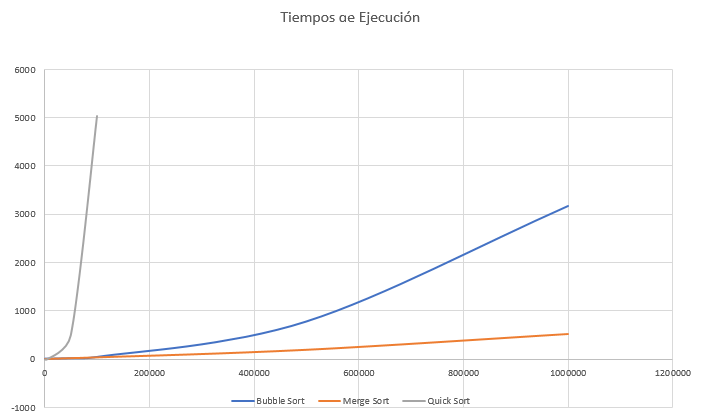
\includegraphics[width=7.05in,height=4.18in]{./media/image1.png}
	\end{Center}
\end{figure}


%%%%%%%%%%%%%%%%%%%% Figure/Image No: 1 Ends here %%%%%%%%%%%%%%%%%%%%

\begin{adjustwidth}{2.67in}{2.79in}
\begin{Center}
{\fontsize{11pt}{13.2pt}\selectfont (Quicksort): O(n log n)\par}
\end{Center}\par

\end{adjustwidth}


\printbibliography
\end{document}